% !TEX program = xelatex
% Краткая версия отчёта для первого контакта с научным руководителем.
\documentclass[11pt]{article}
\usepackage{fontspec}
\setmainfont{Times New Roman}
\usepackage{polyglossia}
\setdefaultlanguage{russian}
\setotherlanguage{english}
\newfontfamily\cyrillicfonttt{Andale Mono}
\usepackage[margin=1in]{geometry}
\usepackage{amsmath,amssymb}
\usepackage{booktabs,longtable,tabularx,array}
\usepackage{graphicx}
\usepackage{caption}
\usepackage{float}
\usepackage{xcolor}
\usepackage{hyperref}
\usepackage{microtype}
\definecolor{ReportBlue}{HTML}{315F72}
\hypersetup{colorlinks=true,linkcolor=black,urlcolor=ReportBlue,citecolor=black}
\graphicspath{{figures/}}
\newcolumntype{Y}{>{\raggedright\arraybackslash}X}
\newcolumntype{P}[1]{>{\raggedright\arraybackslash}p{#1}}
\DeclareRobustCommand{\code}[1]{\texttt{\detokenize{#1}}}
\newcommand{\mae}{\mathrm{MAE}}
\newcommand{\Rtwo}{R^2}
\newcommand{\dd}{\,\mathrm{d}}
\setlength{\parindent}{0pt}
\setlength{\parskip}{0.55\baselineskip}
\setlength{\tabcolsep}{5pt}
\renewcommand{\arraystretch}{1.16}
\captionsetup[figure]{font=small,labelfont=bf,skip=6pt}
\setlength{\textfloatsep}{9pt plus 2pt minus 2pt}
\setlength{\floatsep}{8pt plus 2pt minus 2pt}
\setlength{\intextsep}{8pt plus 2pt minus 2pt}
\frenchspacing

\begin{document}
\sloppy

\title{Краткий отчёт о проделанной работе по проекту TGNN-Solv\\
\large Физически информированная графовая модель для предсказания растворимости}
\author{Поломошнов Никита Львович}
\date{18 апреля 2026 г.}
\maketitle

\section*{Краткое содержание}

В проекте построена и проверена физически информированная графовая модель для предсказания растворимости твёрдых органических соединений в жидких растворителях~\cite{boobier2017,vermeire2022,fastsolv2025}. Этот текст является кратким отчётом о текущем этапе, а не заявлением о завершённом превосходстве физического пути. Целевая величина --- натуральный логарифм мольной доли растворённого вещества в насыщенном растворе,
\begin{equation*}
    y = \ln x_2 .
\end{equation*}

Главная идея модели TGNN-Solv состоит в том, чтобы не предсказывать растворимость напрямую, а провести вычисление через термодинамическое уравнение твёрдо-жидкого равновесия~\cite{prausnitz1998,hildebrand1970}:
\begin{equation}
    \ln x_2 = -\Phi(T) - \ln \gamma_2,
    \qquad
    \Phi(T)=\frac{\Delta G_{\mathrm{fus}}(T)}{RT}.
    \label{eq:sle-short}
\end{equation}
Здесь $\Phi(T)$ описывает вклад плавления чистого твёрдого вещества, а $\gamma_2$ --- коэффициент активности растворённого вещества в растворе. Для честного контроля реализована модель DirectGNN: она использует тот же графовый блок обработки молекул, но предсказывает $\ln x_2$ напрямую, без физического слоя.

\begin{figure}[H]
\centering
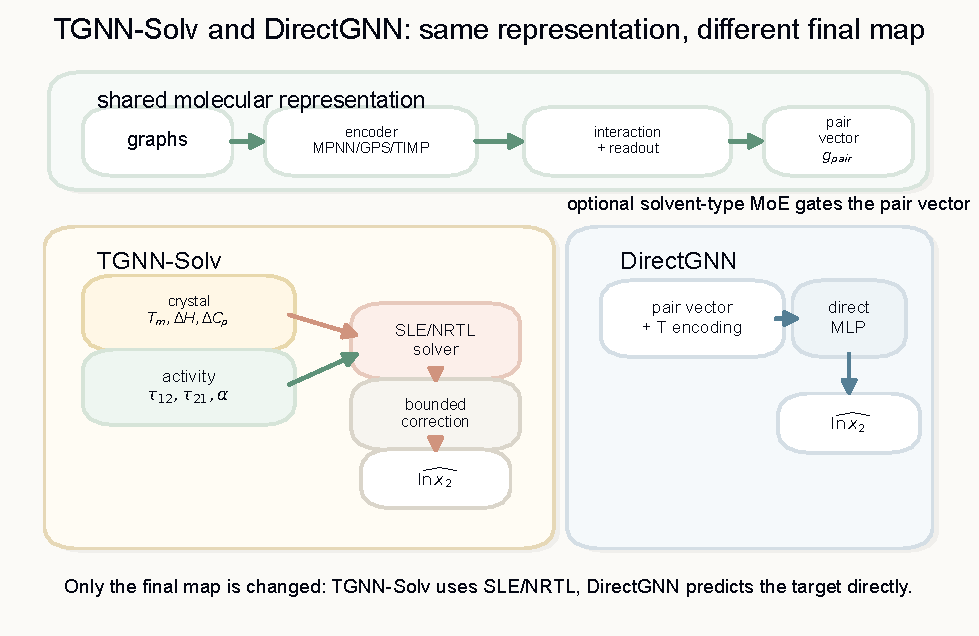
\includegraphics[width=0.96\textwidth]{architecture_schematic.pdf}
\caption{Сравниваемые вычислительные пути. TGNN-Solv проводит предсказание через физические параметры и решатель равновесия; DirectGNN использует тот же молекулярный блок, но предсказывает $\ln x_2$ напрямую.}
\end{figure}

На основном разбиении по новым молекулярным каркасам получено:

\begin{center}
\small
\begin{tabularx}{\textwidth}{P{0.30\textwidth}rrY}
\toprule
Модель & $\mae$ по $\ln x_2$ & $\Rtwo$ & Комментарий \\
\midrule
DirectGNN & 1.652 & 0.478 & лучшая средняя ошибка в одном запуске \\
Случайный лес, гибридные признаки & 1.722 & 0.449 & сильная не нейросетевая проверка \\
TGNN-Solv & 1.741 & 0.438 & физический путь уступает на 0.089 \\
\bottomrule
\end{tabularx}
\end{center}

\begin{figure}[H]
\centering
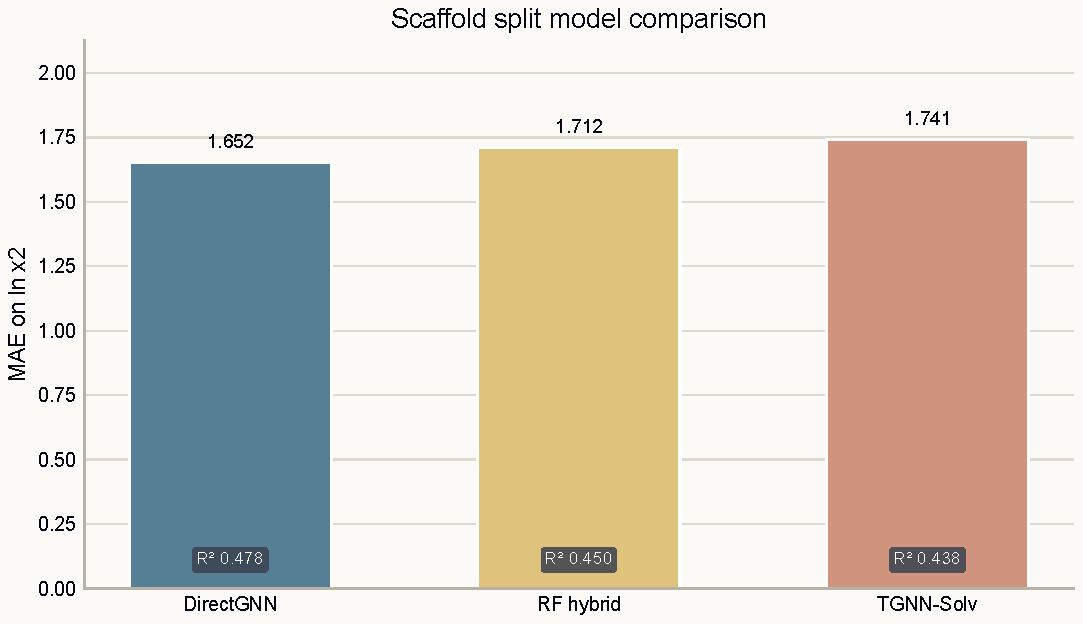
\includegraphics[width=0.86\textwidth]{prediction_slice_model_comparison.pdf}
\caption{Текущее сравнение основных моделей на тестовых срезах. График подчёркивает, что DirectGNN имеет лучшую среднюю ошибку, а TGNN-Solv остаётся близкой, но уступает в этом запуске.}
\end{figure}

Текущий результат требует аккуратной интерпретации. Физическая модель реализована, устойчиво обучается и выигрывает у DirectGNN примерно на $46\%$ тестовых строк. Однако по средней ошибке на новых каркасах она уступает прямой модели. Это означает, что в текущей версии физическое ограничение не даёт выигрыша на основном структурном разбиении. Доверительный интервал для разрыва $0.089$ ещё не оценён, поэтому статистический вывод требует нескольких инициализаций.

Отдельный аудит трудных систем показывает, что часть тяжёлых ошибок связана не только с архитектурой. В каркасном тесте $6.6\%$ строк имеют формальный заряд, $3.6\%$ являются явными солями, $3.5\%$ --- цвиттер-ионами. На нейтральных строках DirectGNN даёт $\mae=1.604$, а TGNN-Solv --- $1.701$; на всех зарядовых строках ошибки возрастают до $2.337$ и $2.309$. На $26$ экстремально плохо растворимых заряженных или антоцианидин-подобных строках ошибка превышает $11$ по $\ln x_2$; $20$ из этих строк приходятся на дельфинидин-хлорид в ацетоне и этаноле. Исходная статья по дельфинидину описывает чистые растворители, но в обработанных строках нет $T_m$ и $\Delta H_{\mathrm{fus}}$, поэтому требуемую активность через кристаллический вклад посчитать нельзя. Поэтому следующий шаг для таких случаев --- аудит кристаллических данных и условий эксперимента, а не немедленное добавление электролитного NRTL.

При этом отдельная температурная проверка показывает, что физический сигнал в данных очень силён. Это именно режим известной пары: аудит подтвердил, что все $1\,751$ пар из высокотемпературного теста присутствуют в низкотемпературной обучающей части. Если для такой пары построить зависимость Вант-Гоффа по низкотемпературным точкам, то высокотемпературные точки предсказываются с ошибкой $\mae=0.368$. Это парно-подогнанный ориентир, а не конкурент для новых химических систем. Краткие локальные запуски нейросетевых моделей существенно хуже: DirectGNN даёт $\mae=1.619$, TGNN-Solv --- $\mae=1.945$. Следовательно, проблема не в отсутствии термодинамического сигнала, а в том, что текущая обучаемая модель не извлекает его из данных достаточно хорошо.

\begin{center}
\small
\begin{tabularx}{\textwidth}{P{0.33\textwidth}P{0.32\textwidth}Y}
\toprule
Утверждение & Основание & Статус \\
\midrule
DirectGNN является сильной контрольной моделью & scaffold split и внешние ориентиры & подтверждено \\
TGNN-Solv платит небольшую цену за физический слой & разница $+0.089$ MAE в одном запуске & диагностировано \\
Температурная физика в данных выражена сильно & Вант-Гофф даёт $\mae=0.368$ & подтверждено \\
Краткий TGNN-запуск не восстанавливает парную активность & почти постоянные NRTL-параметры & диагностировано \\
Полезность новых стабилизирующих компонентов & IDAC, UNIFAC, явные H, TIMP, парные потери & требует планового бюджета \\
\bottomrule
\end{tabularx}
\end{center}


\section{Ключевые термины}

\begin{center}
\begin{tabularx}{\textwidth}{P{0.24\textwidth}Y}
\toprule
Термин & Краткое пояснение \\
\midrule
$\ln x_2$ & Логарифм мольной доли растворяемого вещества; основная целевая величина. \\
Твёрдо-жидкое равновесие & Равенство химических потенциалов вещества в кристалле и насыщенном растворе; физическая основа TGNN-Solv. \\
Графовая модель & Модель, которая читает молекулу как граф атомов и химических связей. \\
Молекулярный каркас & Остов молекулы по Мёрко; разбиение по каркасам проверяет перенос на новые структурные классы. \\
NRTL & Модель коэффициентов активности в неидеальном растворе. \\
IDAC & Коэффициент активности при бесконечном разбавлении; дополнительный прямой сигнал для NRTL-параметров. \\
\bottomrule
\end{tabularx}
\end{center}

\section{Задача}

Для заданных структуры растворяемого вещества, структуры растворителя и температуры требуется предсказать равновесную растворимость в форме $\ln x_2$. Такая величина нужна при выборе растворителя, разработке кристаллизации, очистке вещества и ранней оценке пригодности лекарственных молекул. Экспериментально измерять каждую новую пару вещество--растворитель при нескольких температурах дорого, поэтому расчётная модель полезна только тогда, когда она переносится на новые молекулы и новые температурные области.

Сложность задачи в том, что растворимость зависит и от чистого кристалла, и от жидкой смеси. На кристаллическую часть влияют температура плавления, энтальпия плавления, жёсткость и упаковка молекулы. На часть раствора влияют полярность, водородные связи, донорно-акцепторные свойства, размер молекул и совместимость функциональных групп.

Проект сравнивает два подхода:
\begin{enumerate}
    \item \textbf{TGNN-Solv}: графовая модель предсказывает физические параметры, после чего решается уравнение твёрдо-жидкого равновесия;
    \item \textbf{DirectGNN}: та же графовая обработка молекул, но прямой выход на $\ln x_2$.
\end{enumerate}
Такой контроль нужен, чтобы отделить вклад графового представления от вклада физического ограничения.

\section{Данные}

Основной корпус построен на базе BigSolDB v2.1 и текущих обработанных таблиц проекта~\cite{krasnov2025,bigsoldb2026}. Полные обработанные таблицы содержат $127\,088$ строк; из них $108\,287$ строк имеют целевую растворимость. В подмножестве с метками растворимости есть $1\,525$ уникальных растворяемых веществ, $212$ растворителей и $12\,129$ уникальных пар. Температуры лежат в диапазоне $243.15$--$425.77\,\mathrm{K}$, медианная температура равна $303.15\,\mathrm{K}$.

Подготовка данных была самостоятельной частью работы. Все записи приводятся к единому контракту: канонические SMILES, температура в Кельвинах, целевая величина $\ln x_2$, явные маски для отсутствующих физических меток и сохранение происхождения строк. Это позволяет обучать модель на разреженной физической разметке без подстановки нулей вместо отсутствующих значений.

\begin{center}
\begin{tabular}{lr}
\toprule
Показатель & Значение \\
\midrule
Все строки в обработанных таблицах & $127\,088$ \\
Строки с целевой растворимостью & $108\,287$ \\
Уникальные растворяемые вещества с метками растворимости & $1\,525$ \\
Уникальные растворители с метками растворимости & $212$ \\
Уникальные пары с метками растворимости & $12\,129$ \\
Диапазон температур & $243.15$--$425.77\,\mathrm{K}$ \\
Среднее число строк на пару & $8.93$ \\
Медианное число температурных строк на пару & $9$ \\
Дубликаты троек вещество--растворитель--температура & $0$ \\
\bottomrule
\end{tabular}
\end{center}

Основной режим оценки --- разбиение по молекулярным каркасам растворяемого вещества. Это строгий режим: модель должна работать на новых структурных классах, а не просто интерполировать между уже виденными строками.

Отдельно собран корпус IDAC --- коэффициентов активности при бесконечном разбавлении. Стартовый набор был не частью BigSolDB, а отдельным ThermoML-корпусом: $9$ вручную выбранных DOI из \code{idac_seed_dois.txt}, официальные NIST ThermoML JSON-записи, фильтрация бинарных жидкофазных IDAC-измерений, перевод InChI в SMILES через RDKit и сохранение $\gamma^\infty$, $\ln\gamma^\infty$, метода, фазы, стандартного состояния и DOI-источника~\cite{idac_zenodo,frenkel2006,nist_thermoml}. Он содержал $404$ экспериментальные строки и $138$ пар. Для расширения был реализован извлекатель из NIST ThermoML: он находит DOI в архиве, загружает ThermoML JSON, выбирает бинарные измерения $\gamma^\infty$, переводит структуры в SMILES через RDKit, считает $\ln\gamma^\infty$ и агрегирует дубликаты по паре и температуре. Итоговый расширенный корпус содержит $14\,900$ строк, $3\,145$ пар, $136$ растворяемых веществ, $112$ растворителей и $63$ DOI; конфликтующих агрегированных групп не найдено. Точное пересечение с SLE-парами и SLE-тройками равно $0\%$, поэтому эти данные не являются утечкой растворимости.

IDAC подключается не как строки растворимости, а отдельным обучающим потоком с маской активности. Это принципиально: IDAC измеряет предел активности, а не насыщенную растворимость. Его роль --- ограничить NRTL-ветвь и уменьшить компенсаторную неоднозначность между кристаллическим вкладом и активностью раствора.

Вода сохранена в корпусе как растворитель. Для неё реализован отдельный режим графового представления с явными водородами: вместо одноузлового графа $\mathrm{O}$ используется граф $\mathrm{H{-}O{-}H}$. Это устраняет вырожденный случай, в котором передача сообщений по химическим связям почти не работает~\cite{gilmer2017,landrum2024}.

\begin{figure}[H]
\centering
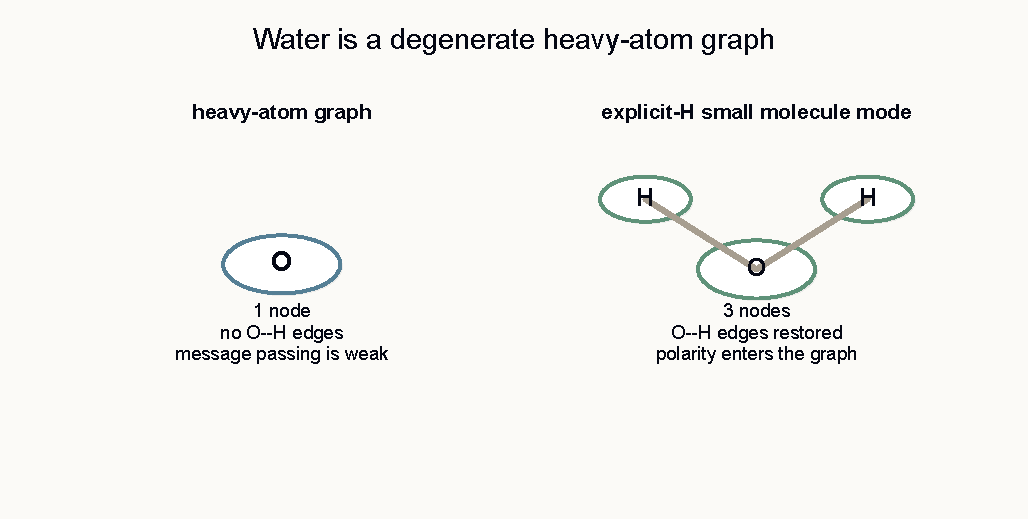
\includegraphics[width=0.92\textwidth]{water_graph_schematic.pdf}
\caption{Исправление графа воды и малых молекул: явные водороды возвращают O--H связи в граф и дают модели доступ к полярной структуре молекулы.}
\end{figure}


\section{Контекст сравнения}

TGNN-Solv сопоставляется не только с собственной прямой моделью DirectGNN. В проекте поддерживаются также случайный лес на молекулярных признаках и внешние ориентиры SolProp и FastSolv~\cite{vermeire2022,fastsolv2025}. Это важно методически: если DirectGNN находится на уровне внешних моделей, то качество данных и графового представления в целом достаточно сильное; тогда отставание TGNN-Solv следует искать в физическом пути, а не в общей инфраструктуре.

Классы методов различаются по смыслу. Дескрипторные модели и прямые графовые модели обычно дают один численный ответ~\cite{gilmer2017,yang2019}. Термодинамические модели вроде NRTL и UNIFAC описывают коэффициенты активности, но требуют параметров или покрытия функциональных групп~\cite{renon1968,fredenslund1975,weidlich1987}. TGNN-Solv пытается объединить эти подходы: графовая часть предсказывает параметры, а физическое уравнение задаёт форму итогового расчёта.

\section{Термодинамическая постановка}

В равновесии химический потенциал растворяемого вещества в твёрдой фазе равен химическому потенциалу в жидком растворе~\cite{prausnitz1998,hildebrand1970}. Для раствора:
\begin{equation*}
    \mu_2^{\mathrm{liq}}(T,P,x)
    = \mu_2^{\mathrm{liq},0}(T,P) + RT\ln(\gamma_2 x_2).
\end{equation*}
После введения свободной энергии плавления
\begin{equation*}
    \Delta G_{\mathrm{fus}}(T)
    = \mu_2^{\mathrm{liq},0}(T)-\mu_2^{\mathrm{sol},0}(T)
\end{equation*}
получается уравнение \eqref{eq:sle-short}. В приближении $\Delta C_p^{\mathrm{fus}}=0$ кристаллический вклад равен
\begin{equation*}
    \Phi(T)
    = \frac{\Delta H_{\mathrm{fus}}}{R}\left(\frac{1}{T}-\frac{1}{T_{\mathrm m}}\right).
\end{equation*}
Для активности используется модель NRTL с параметрами $\tau_{12}$, $\tau_{21}$ и $\alpha$~\cite{renon1968}. При бесконечном разбавлении:
\begin{equation*}
    \ln \gamma_2^{\infty}
    = \tau_{12} + \tau_{21}\exp(-\alpha \tau_{21}).
\end{equation*}
Эта формула используется для подключения IDAC-данных.

\begin{figure}[H]
\centering
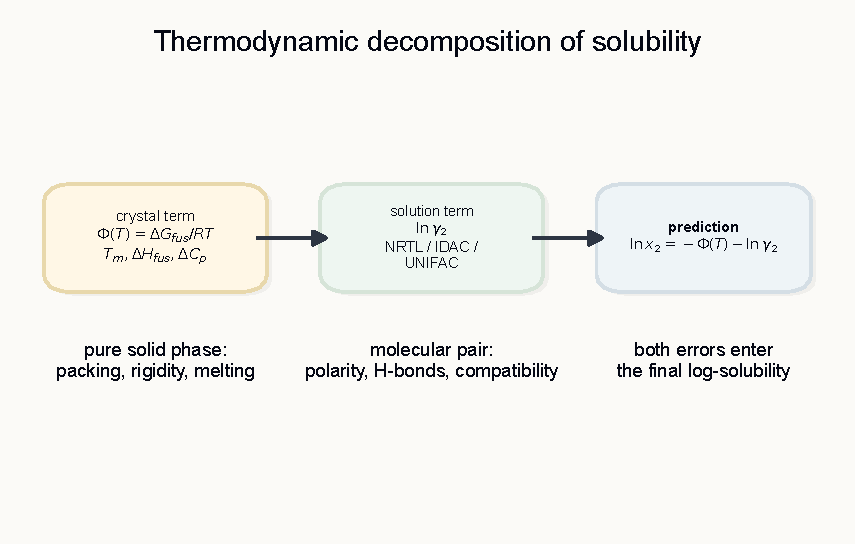
\includegraphics[width=0.92\textwidth]{sle_decomposition_schematic.pdf}
\caption{Разложение предсказания растворимости на кристаллический вклад $\Phi(T)$ и вклад активности $-\ln\gamma_2$. Именно это разложение делает промежуточные параметры физически проверяемыми.}
\end{figure}

\section{Что реализовано}

Реализованы полный путь TGNN-Solv, контрольная DirectGNN, решатель равновесия, несколько режимов графового кодирования молекул, обработка воды с явными водородами, расширенный обучающий сигнал по коэффициентам активности при бесконечном разбавлении, UNIFAC-псевдометки, температурные разбиения, внешние сравнения с SolProp и FastSolv, а также диагностические программы для анализа ошибок.

Архитектура включает больше, чем один стандартный графовый блок. Базовый MPNN дополняется опциональными вариантами GPS/GraphGPS и TIMP: первый добавляет глобальное внимание, второй разделяет сообщения на дисперсионный и полярно-ассоциативный каналы. Для построения пары используется перекрёстное внимание, после которого возможна остаточная смесь экспертов по типу растворителя. Итоговая коррекция в TGNN-Solv тоже остаётся физической: модель предлагает ограниченные поправки к параметрам и повторно решает SLE, а не добавляет свободный сдвиг к $\ln x_2$.

В части данных реализованы не только финальные таблицы, но и воспроизводимые программы: подготовка основных разбиений, извлечение IDAC из ThermoML, построение отдельного IDAC-потока, UNIFAC-псевдометки, температурные разбиения и диагностические аудиты.

\section{Как обучается модель}

TGNN-Solv обучается не одним шагом, а поэтапно. Сначала возможен этап предобучения графового блока: восстановление маскированных атомов и связей, предсказание RDKit-дескрипторов и контрастивная задача на разных представлениях одной молекулы. Этот этап нужен для химически осмысленной инициализации, но сам по себе не решает задачу совместимости вещества и растворителя; поэтому отдельно подготовлены парные задачи, контрастивное выравнивание по параметрам Хансена и диагностика каналов TIMP.

Основное обучение состоит из трёх фаз. В первой фазе сильнее используются вспомогательные физические свойства: $T_m$, $\Delta H_{\mathrm{fus}}$, параметры Хансена и IDAC. Во второй фазе включается полный SLE-путь и доминирует ошибка по растворимости. Третья фаза выполняет тонкую настройку с меньшим шагом. Такой порядок нужен, чтобы случайные начальные NRTL-параметры не ломали решатель и не давали бессмысленные градиенты.

Функция ошибки складывается из основной ошибки Хьюбера по $\ln x_2$ и вспомогательных физических членов:
\begin{equation*}
    \mathcal L
    = \lambda_{\mathrm{sol}}\mathcal L_{\mathrm{sol}}
    + \lambda_{\mathrm{cryst}}\mathcal L_{\mathrm{cryst}}
    + \lambda_{\mathrm{IDAC}}\mathcal L_{\mathrm{IDAC}}
    + \lambda_{\mathrm{temp}}\mathcal L_{\mathrm{temp}}
    + \lambda_{\mathrm{reg}}\mathcal L_{\mathrm{reg}}.
\end{equation*}
Здесь отсутствующие метки маскируются, а IDAC используется только как отдельный сигнал для коэффициентов активности. Это принципиально: IDAC не является строкой растворимости и не должен искусственно добавляться в SLE-таблицу. В ранних версиях также были проверены более агрессивные физические штрафы: мостовой компонент оказался потенциально опасным для систем с водородными связями, а локальный штраф Вант-Гоффа требовал стабилизации масштаба, чтобы не подавлять основную ошибку по растворимости.

\section{Основные результаты}

Разные разбиения показывают, что главная трудность --- перенос на новые растворяемые вещества и новые каркасы:

\begin{center}
\begin{tabular}{lrrl}
\toprule
Разбиение & $\mae$ & $\Rtwo$ & Вывод \\
\midrule
Случайные строки & 0.166 & 0.987 & слишком лёгкий режим \\
Случайные пары & 0.783 & 0.806 & компоненты обычно уже видны \\
Новый растворитель & 0.732 & 0.735 & относительно легче \\
Новое вещество & 1.642 & 0.420 & основная сложность \\
Новый каркас & 1.703 & 0.462 & новая структура и смещение распределения \\
\bottomrule
\end{tabular}
\end{center}

Внешние сравнения подтверждают уровень прямой графовой модели. SolProp при переобучении на тех же целевых величинах на разбиении по новым веществам даёт $\mae=1.624$ и $\Rtwo=0.388$; DirectGNN имеет близкую $\mae=1.652$, но более высокий $\Rtwo=0.478$. FastSolv после исправления проблем с преобразованием единиц запускается корректно, но остаётся слабее: $\mae=1.941$, $\Rtwo=0.226$.

Температурная экстраполяция даёт наиболее важный физический результат. Протокол был дополнительно проверен: низкотемпературная обучающая и высокотемпературная тестовая части имеют $100\%$ пересечение пар; вода составляет $12.2\%$ тестовых строк; положительный сдвиг растворимости при переходе к высоким температурам наблюдается у $99.6\%$ пар. Поэтому слабость нейросетевых кратких запусков нельзя объяснить тем, что тест состоит в основном из воды или систем с обратным температурным трендом.

\begin{center}
\begin{tabular}{lrrr}
\toprule
Метод & $\mae$ & $\Rtwo$ & Правильное направление \\
\midrule
Вант-Гофф для каждой пары & 0.368 & 0.887 & 99.0\% \\
Линейная зависимость от $T$ & 0.414 & 0.850 & 99.0\% \\
Случайный лес с температурой & 1.290 & 0.658 & 40.4\% \\
DirectGNN, краткий запуск & 1.619 & 0.283 & --- \\
TGNN-Solv, краткий запуск & 1.945 & 0.060 & --- \\
\bottomrule
\end{tabular}
\end{center}

\begin{figure}[H]
\centering
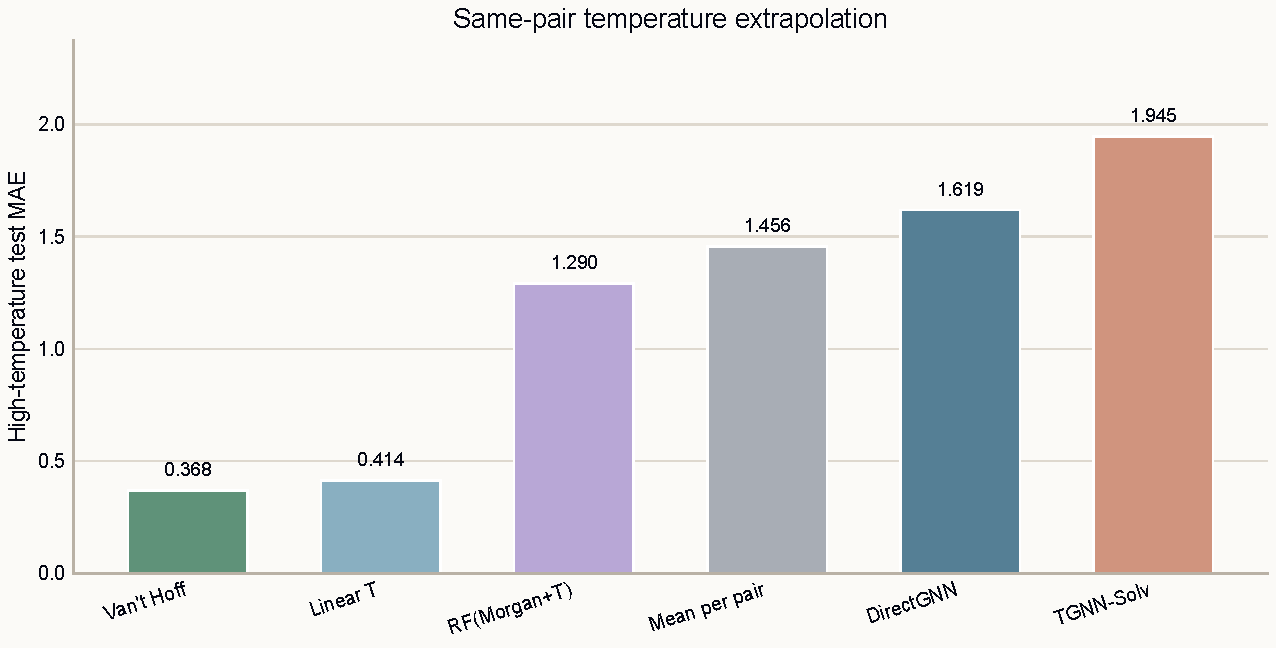
\includegraphics[width=0.88\textwidth]{temperature_extrapolation_baseline_comparison.pdf}
\caption{Температурная экстраполяция внутри известной пары. Аналитическая форма Вант-Гоффа резко превосходит нейросетевые краткие запуски, что является главным аргументом в пользу полноценной проверки физического пути.}
\end{figure}

Этот результат показывает, что термодинамическая форма зависимости от температуры действительно содержится в данных. При этом Вант-Гофф в этой таблице является парно-подогнанным ориентиром, а не честным конкурентом для прогноза новых пар: он явно использует низкотемпературные точки той же пары. Следующий научный вопрос --- может ли TGNN-Solv при плановом обучении приблизиться к этому физическому пределу и использовать температурную форму лучше прямой модели.

Дополнительная диагностика показала, где именно ломается краткий запуск TGNN-Solv. На парах с как минимум тремя высокотемпературными точками медианная ошибка наклона $\ln x_2$ от $1/T$ равна $763\,\mathrm{K}$ для парной аппроксимации Вант-Гоффа, $1\,158\,\mathrm{K}$ для TGNN-Solv и $1\,630\,\mathrm{K}$ для DirectGNN. При этом общая ошибка TGNN-Solv всё равно хуже: $\mae=1.945$. Причина видна во внутренних величинах: стандартное отклонение предсказаний TGNN-Solv составляет только $0.582$ при истинном $2.560$, $\tau_{12}$ почти не меняется от пары к паре ($\sigma\approx4.8\cdot10^{-5}$), а средняя финальная поправка к физическому выходу равна всего $1.1\cdot10^{-5}$. То есть в этом коротком запуске NRTL-ветвь фактически не выучила парную активность, а модель даёт слишком сжатый набор температурных кривых.

\begin{figure}[H]
\centering
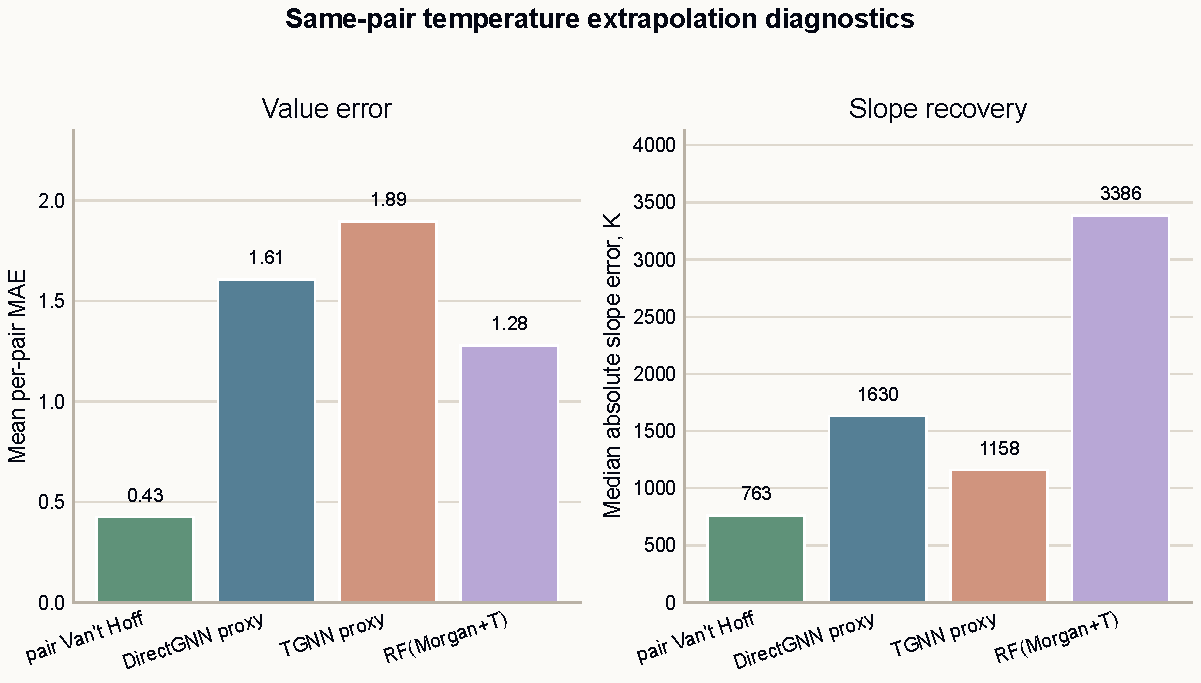
\includegraphics[width=0.92\textwidth]{temperature_slope_recovery_diagnostics.pdf}
\caption{Диагностика значения и наклона на температурной экстраполяции. Краткий запуск TGNN-Solv частично восстанавливает знак и масштаб наклона, но проигрывает по уровню $\ln x_2$ и даёт слишком сжатые предсказания.}
\end{figure}

Дополнительно реализованы прикладные и диагностические слои: быстрое применение модели, температурное сканирование, ранжирование растворителей и оценка технологического окна. Отдельно поддержаны оценка неопределённости через случайное выключение нейронов или ансамбли и проверка области применимости по расстоянию в пространстве скрытых представлений и сходству отпечатков Моргана по Танимото. Эти блоки не подменяют научное сравнение моделей, но показывают, что проект доведён до воспроизводимого исследовательского контура.


\section*{Итог}

К настоящему моменту выполнена основная методическая и программная часть проекта: подготовлены данные, реализованы две сопоставимые модели, проведены внешние сравнения, проверены температурные режимы и разобраны основные источники ошибки. DirectGNN лучше TGNN-Solv по средней ошибке на новых каркасах в одном поддерживаемом запуске, но температурные эксперименты показывают сильный физический сигнал, который текущая обучаемая TGNN-Solv не использует полностью. Последняя диагностика делает это утверждение конкретным: в кратком запуске TGNN-Solv почти не варьирует NRTL-параметры по парам, поэтому физическая часть раствора не несёт достаточной химической информации.

Главный результат этого этапа состоит в уточнении научного вопроса. Теперь нужно проверить не абстрактную идею «добавить физику», а конкретную гипотезу: сможет ли физический путь при плановом обучении восстановить температурную структуру данных лучше прямой модели, не теряя при этом качества на новых молекулярных каркасах.

\begin{thebibliography}{99}

\bibitem{krasnov2025} Krasnov, L., Malikov, D., Kiseleva, M., Tatarin, S., Sosnin, S., Bezzubov, S. BigSolDB 2.0, dataset of solubility values for organic compounds in different solvents at various temperatures. \textit{Scientific Data}, 2025. \url{https://doi.org/10.1038/s41597-025-05559-8}

\bibitem{bigsoldb2026} BigSolDB 2.1: A Comprehensive Dataset of Solubility Values for Organic Compounds in Organic Solvents and Water at Various Temperatures. Zenodo, 2026. \url{https://zenodo.org/records/15094979}

\bibitem{prausnitz1998} Prausnitz, J. M., Lichtenthaler, R. N., de Azevedo, E. G. \textit{Molecular Thermodynamics of Fluid-Phase Equilibria}. 3rd ed. Prentice Hall, 1998.

\bibitem{hildebrand1970} Hildebrand, J. H., Prausnitz, J. M., Scott, R. L. \textit{Regular and Related Solutions}. Van Nostrand Reinhold, 1970.

\bibitem{renon1968} Renon, H., Prausnitz, J. M. Local compositions in thermodynamic excess functions for liquid mixtures. \textit{AIChE Journal}, 14(1), 135--144, 1968. \url{https://doi.org/10.1002/aic.690140124}

\bibitem{fredenslund1975} Fredenslund, A., Jones, R. L., Prausnitz, J. M. Group-contribution estimation of activity coefficients in nonideal liquid mixtures. \textit{AIChE Journal}, 21(6), 1086--1099, 1975. \url{https://doi.org/10.1002/aic.690210607}

\bibitem{weidlich1987} Weidlich, U., Gmehling, J. A modified UNIFAC model. 1. Prediction of VLE, hE, and gamma-infinity. \textit{Industrial \& Engineering Chemistry Research}, 26(7), 1372--1381, 1987. \url{https://doi.org/10.1021/ie00067a018}

\bibitem{idac_zenodo} TGNN-Solv External IDAC Starter Corpus. Zenodo, 2026. Files: \code{idac.csv}, \code{idac_seed_dois.txt}. \url{https://zenodo.org/records/19484205}

\bibitem{frenkel2006} Frenkel, M., Chirico, R. D., Diky, V., et al. XML-Based IUPAC Standard for Experimental, Predicted, and Critically Evaluated Thermodynamic Property Data Storage and Capture (ThermoML). \textit{Pure and Applied Chemistry}, 78(3), 541--612, 2006. \url{https://doi.org/10.1351/pac200678030541}

\bibitem{nist_thermoml} National Institute of Standards and Technology. ThermoML Archive. \url{https://www.nist.gov/mml/acmd/trc/thermoml/thermoml-archive}

\bibitem{landrum2024} Landrum, G. RDKit: Open-source cheminformatics software, 2024. \url{https://www.rdkit.org}

\bibitem{gilmer2017} Gilmer, J., Schoenholz, S. S., Riley, P. F., Vinyals, O., Dahl, G. E. Neural message passing for quantum chemistry. \textit{Proceedings of ICML}, 2017. \url{https://proceedings.mlr.press/v70/gilmer17a.html}

\bibitem{yang2019} Yang, K., Swanson, K., Jin, W., et al. Analyzing learned molecular representations for property prediction. \textit{Journal of Chemical Information and Modeling}, 59(8), 3370--3388, 2019. \url{https://doi.org/10.1021/acs.jcim.9b00237}

\bibitem{boobier2017} Boobier, S., Hose, D. R. J., Blacker, A. J., Nguyen, B. N. Machine learning with physicochemical relationships: solubility prediction in organic solvents and water. \textit{Nature Communications}, 8, 1600, 2017. \url{https://doi.org/10.1038/s41467-017-01920-0}

\bibitem{vermeire2022} Vermeire, F. H., Chung, Y., Green, W. H. Predicting solubility limits of organic solutes for a wide range of solvents and temperatures. \textit{Journal of the American Chemical Society}, 144(24), 10785--10797, 2022. \url{https://doi.org/10.1021/jacs.2c01768}

\bibitem{fastsolv2025} Attia, L., Burns, J. W., Doyle, P. S., et al. Data-driven organic solubility prediction at the limit of aleatoric uncertainty. \textit{Nature Communications}, 16, 7497, 2025. \url{https://doi.org/10.1038/s41467-025-62717-7}

\end{thebibliography}


\end{document}
